\documentclass[12pt]{article} \usepackage{COSC420style} \usepackage{soul}

\usepackage{verbatim}
\usepackage{graphicx}
\usepackage{subcaption}
\papercode{COSC420}

\title{Transformer based language model}

\author{Jake \textsc{Norton}} \studentid{5695756}

\reportdate{\today}

\begin{document}

\maketitle

\section{Introduction}

I have created a framework to generate text both from a combination of Pride and Predjudice and War
and Peace as the datasets. Many of the decisions made here were close to arbitrary in nature due to
time constraints, and I did not get to explore as much as I would have liked. However, I do believe
that the models created are still adequate at creating text that is at least interesting. In terms
of text choice, I decide to use all of both books. This provided the most data, but at a cost of
potential bias. This was a trade off I was willing to take as I hoped that generally the model would
perform better, if skewed towards talking about war and peace

\section{Task 1: Tok2Vec Encoder}

\subsection{Methodology}

There are two general approaches taken to create word2vec embeddings, Skip-gram(SG) and continuous bag
of words(CBOW). They are inverses of each other, CBOW is designed to predict a word given its
surrounding context words. SG therefore from a given word tries to predict its context, ie, the
words surrounding it. Generally, CBOW works well in contexts where the emphasis is finding common
connections between common words. For a small dataset this is useful as it is looking for more
simple relationships, and so needs less data to find them. However the averaging which occurs over
all of the context can result in a less nuanced view. Skip-gram however tends to pick up more
complicated relationships at the cost of needing more time and more data to train, it needs to train
separately for each position in the conteaxt window to be effective, whereas CBOW can add all the
context at once. I decided to use Skip-gram as I thought it would be more interesting to see if it
could still perform ok given the dataset constraints. Part of the reason for the lack of exploration
in the process was due to a corruption of my early token-to-vector models. In order to speed up the
process I decided to save the encoded vectors of the entire corpus, and simply read it in each time.
This did significantly improve the time taken, however somewhere along the line this dataset was
corrupted. When looking at the TNE plots of the models, they seem like they are doing somewhat what
is expected, creating clusters around semantically similar words. However, as I found out later,
when running a prediction on these models, the output would be all the same, some combination of

\begin{itemize}
	\item I
	\item /ae
	\item =
\end{itemize}

This rendered the resulting transformer models to produce garbled output as well.
Below is the hyperparameters I used in the end for my token-to-vector model. In terms of context
window, anything below 3 didn't give me good outcomes when it came to the prediction test, I went up
to 5, choosing between 3,4 and 5 was difficult, mainly the difference was that the higher the
context window, the higher it priorized punctuation. As the decision became somewhat arbitrary I
decided to go with 4 in the hope of splitting the difference as well as reduction in training time.
I am happy in the end with the split of punctuation vs text, however quotations are still a point
that the model often struggles with. Additionally the models with context windows of 4 tended to
have a nice evenish distribution, with some notable clustering with expected semantically similar
words like "would, should , could, must, shall".
% [here is ctx window 1 as example dim_32_ctx_1_embedding.svg]

\begin{figure}[htbp]
	\centering
	\begin{subfigure}[b]{0.45\textwidth}
		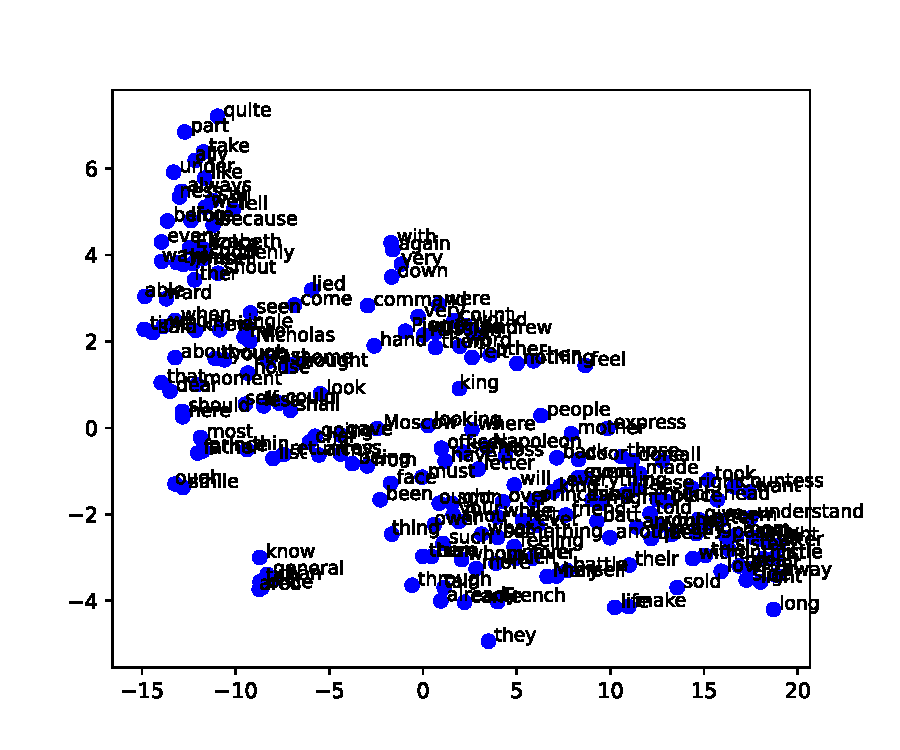
\includegraphics[width=\textwidth]{./figures/dim_32_ctx_1_embedding.pdf}
		\caption{hidden layers: 32, context window of 1}
		\label{fig:32_1}
	\end{subfigure}
	\begin{subfigure}[b]{0.45\textwidth}
		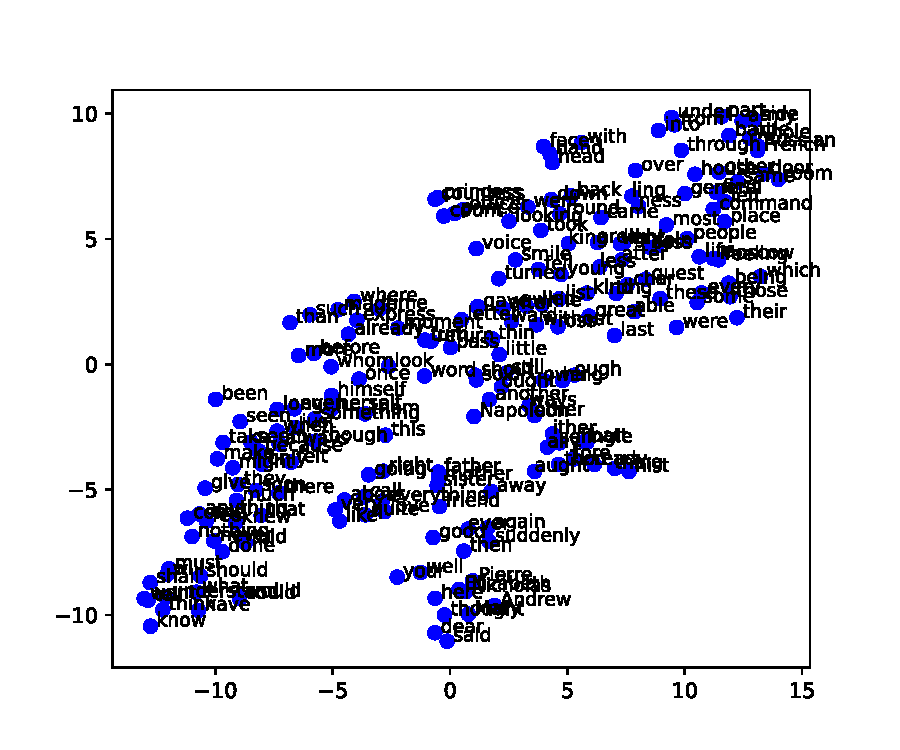
\includegraphics[width=\textwidth]{./figures/dim_32_ctx_4_embedding.pdf}
		\caption{hidden layers: 32, context window of 4}
		\label{fig:32_4}
	\end{subfigure}
	\newline % starts a new line
	\begin{subfigure}[b]{0.45\textwidth}
		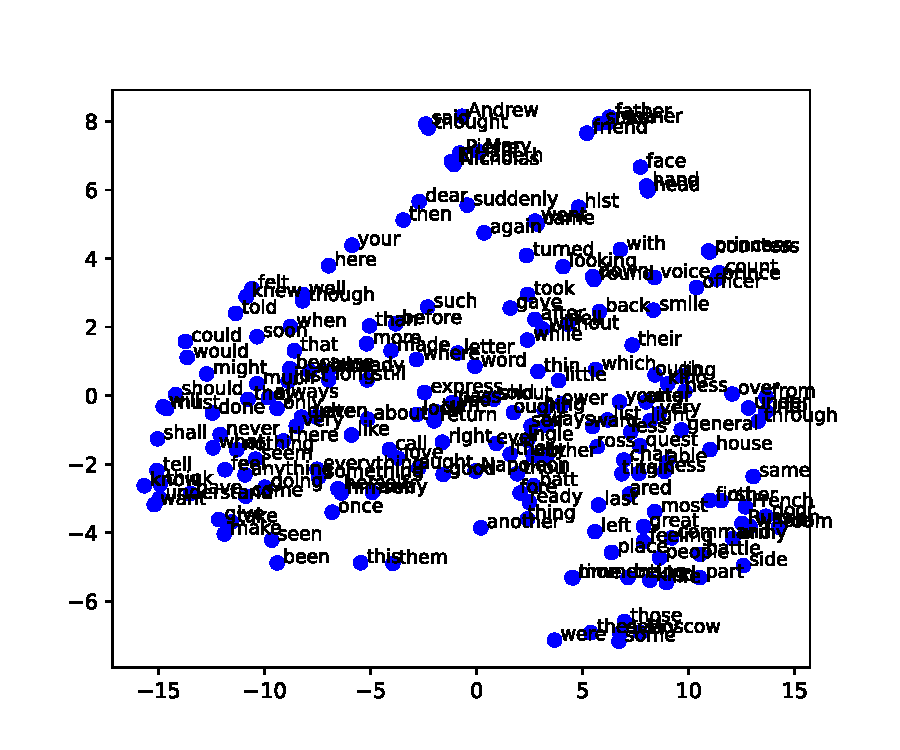
\includegraphics[width=\textwidth]{./figures/dim_64_ctx_3_embedding.pdf}
		\caption{hidden layers: 64, context window of 3}
		\label{fig:64_3}
	\end{subfigure}
	\begin{subfigure}[b]{0.45\textwidth}
		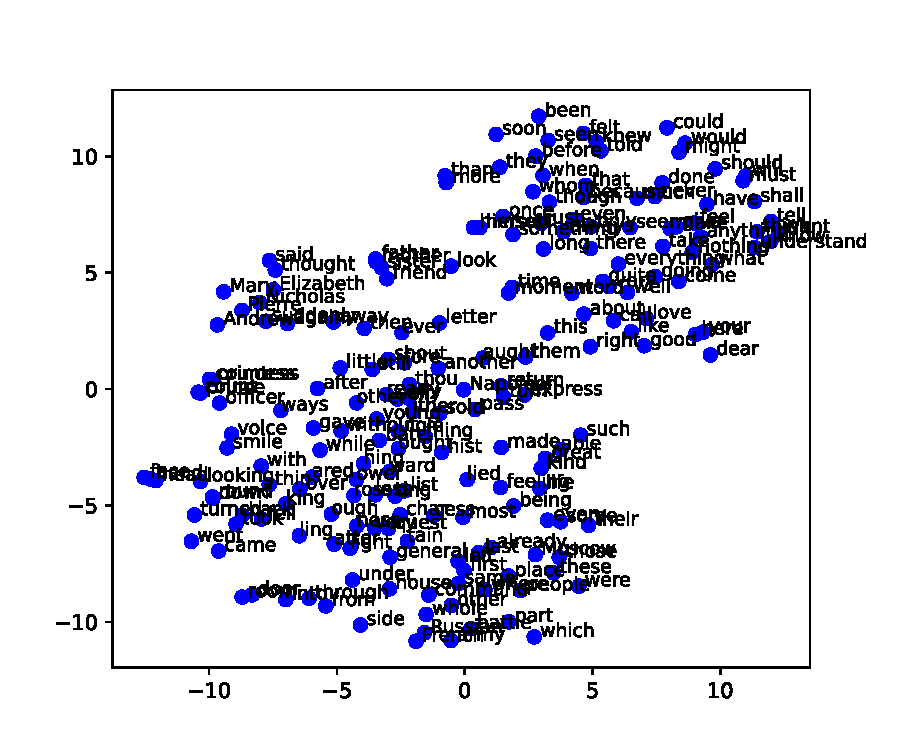
\includegraphics[width=\textwidth]{./figures/dim_64_ctx_5_embedding.pdf}
		\caption{hidden layers: 64, context window of 5}
		\label{fig:64_5}
	\end{subfigure}
	\caption{t-SNE plots of embedding space with varying sizes of hidden layers and context
		windows}
	\label{fig:small_embeddings}
\end{figure}

\begin{figure}[htbp]
	\centering
	\begin{subfigure}[b]{0.45\textwidth}
		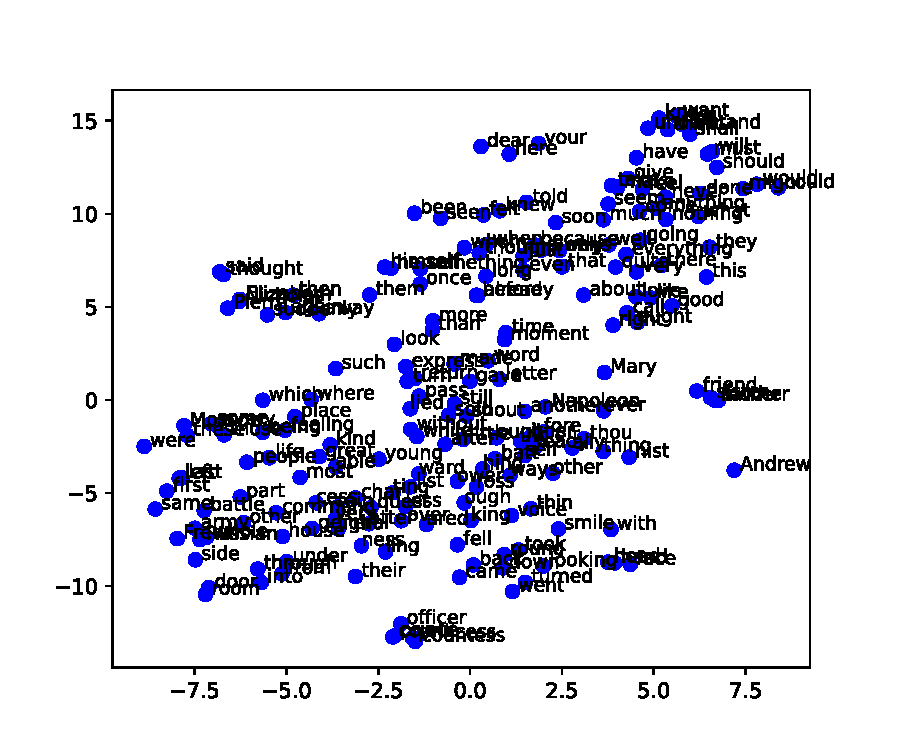
\includegraphics[width=\textwidth]{./figures/dim_64_ctx_4_embedding.pdf}
		\caption{hidden layers: 64, context window: 4}
		\label{fig:64_4}
	\end{subfigure}
	\hfill % Add horizontal space between the first and second subfigures on the same row
	\begin{subfigure}[b]{0.45\textwidth}
		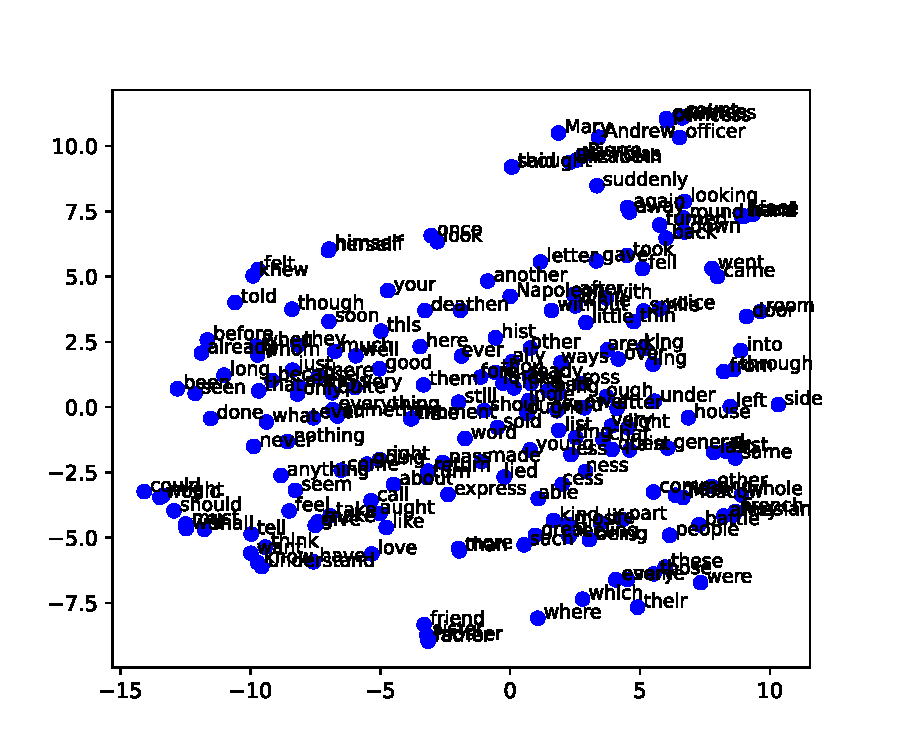
\includegraphics[width=\textwidth]{./figures/dim_128_ctx_4_embedding.pdf}
		\caption{hidden layers: 128, context window: 4}
		\label{fig:128_4}
	\end{subfigure}
	\newline % Starts a new line for the next row: subfigures
	\begin{subfigure}[b]{0.45\textwidth}
		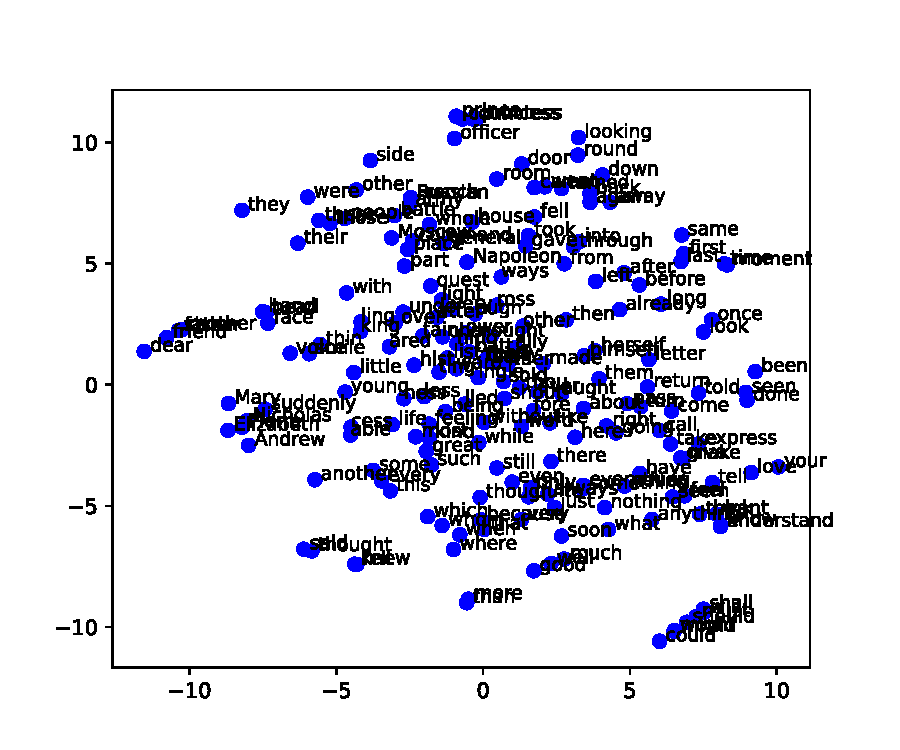
\includegraphics[width=\textwidth]{./figures/dim_256_ctx_4_embedding.pdf}
		\caption{hidden layers: 256, context window: 4}
		\label{fig:256_4}
	\end{subfigure}
	\hfill % Add horizontal space between the first and second subfigures on the same row
	\begin{subfigure}[b]{0.45\textwidth}
		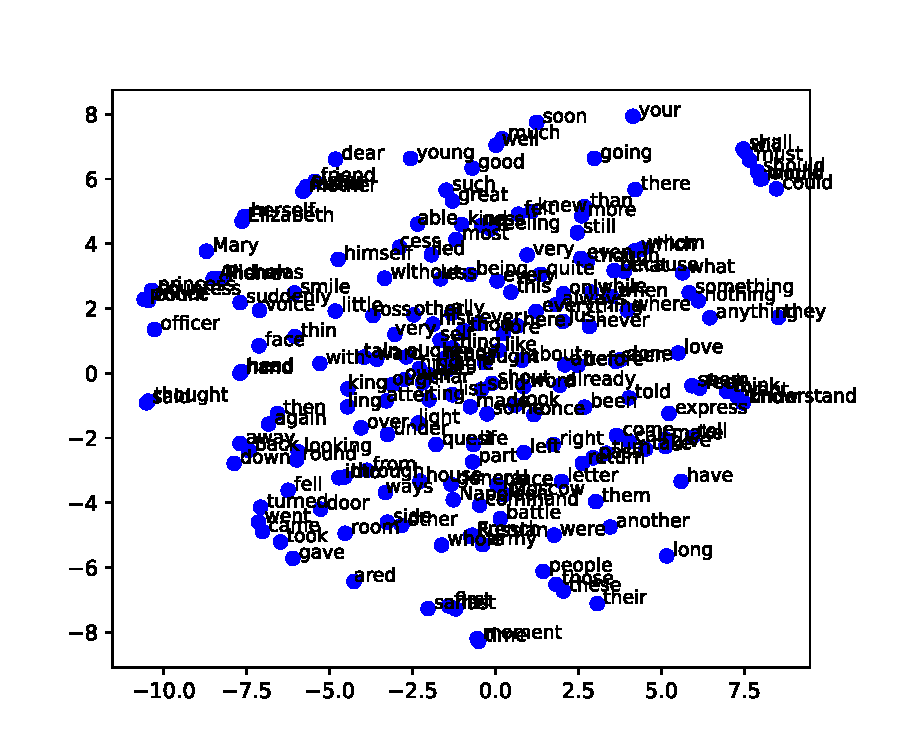
\includegraphics[width=\textwidth]{./figures/dim_512_ctx_4_embedding.pdf}
		\caption{hidden layers: 512, context window: 4}
		\label{fig:512_4}
	\end{subfigure}
	\caption{t-SNE plots of embedding space with varying sizes of hidden layers and context windows}
	\label{fig:larger_embeddings}
\end{figure}

To find out the vocab size I calculated a rough count of unique words\footnote{bash command:
\texttt{tr '[:upper:]' '[:lower:]' < combined\_books\_text | tr -d '[:punct:]' | tr ' '
'\textbackslash{}n' | sort | uniq | wc -l}} over the whole corpus which gave me approximately 25,000
words. From the eye test, though, there were many duplicates/close duplicates in there, mainly due
to punctuation, for example.

\begin{itemize}
	\item   ‘your
	\item   “your
	\item   your
	\item   “you’re
	\item   you’re
\end{itemize}

To capture as much as I could I went up to 5000 tokens which was the limit due to memory and model
size concerns at higher token counts. Additionally, if chatgpt can manage with only ~50000 unique
tokens, 10\% for a corpus of this size seems reasonable to me.

I tested a range of values for the the hidden layer dimension, from 32 up to 512. From my findings
again with limited testing it was hard to quantitatively decide which would be the best to continue
with. For sure I could tell that 32 and 64 were not enough as there was a heavy skew present in the
graphs output from all of these dimensions. Due to how t-SNE squishes the dimensionality, I am not
sure that having a linear skew is necessarily a bad thing, however my interpretation was that the
skewness represented a simpler embedding representation.

I chose to go with the middle of the good values again.

\begin{itemize}
	\item \textbf{Context Window}: 4
	\item \textbf{Hidden Layer Dimension}: 256
	\item \textbf{Vocab Size}: 5000
\end{itemize}

\subsection{Implementation}

\subsection{Results}

Visualization of the vector embeddings using t-SNE and K-means clustering, along with a discussion
on the distinctiveness and coverage of the vector space.

\section{Task 2: Transformer-based Text Prediction}

\subsection{Methodology}

Description of the transformer model architecture, including the choice of hyperparameters such as
sequence size, number of layers, self-attention heads, and neurons in the dense network.

\subsection{Implementation}

Discussion on the implementation details, training process, and the challenges encountered during
the model training.

\subsection{Results}

Analysis of training and, if applicable, validation accuracies. Qualitative assessment of the text
generation capabilities for both the one-hot encoded and Tok2Vec encoded models. Comparison of
outputs when prompted with extracts from the training texts versus new, unseen prompts.

\section{Task 3: Report and Evaluation}

\subsection{Overview of Tasks}

Summary of the methodologies and key decisions taken during the project.

\subsection{Evaluation and Comparison}

Critical evaluation of the models based on the tasks' results, discussing the effectiveness and
limitations of each approach.

\section{Conclusion}

Reflections on the project outcomes, lessons learned, and potential areas for future research.

\section{References}
% Use BibTeX or a manually curated bibliography.

\end{document}
